\documentclass[12pt, a4paper]{article}
\usepackage[utf8]{inputenc}
\usepackage{graphicx}
\usepackage{gensymb}
\usepackage{amsmath}
\usepackage{float}
\usepackage[figurename=Graf]{caption}
\usepackage{subcaption}

\title{Airyjevi funkciji}
\author{Miha Pompe}
\date{Oktober 2021}

\begin{document}
\begin{titlepage}
	\centering
 	
\includegraphics[width=0.45\textwidth]{logo_fmf_uni-lj_sl_veliki.png}\par\vspace{1cm}

	\vspace{1cm}

	\vspace{1.5cm}
	{\huge\bfseries Airyjevi funkciji\par}
	\vspace{2cm}
	{\Large Miha Pompe 28191072\par}
	\vfill

	\vfill

% Bottom of the page
	{\large Oktober 2021\par}
\end{titlepage}
% \maketitle
\thispagestyle{empty}
\clearpage
\pagenumbering{arabic}
\newpage


\section{Uvod}
Airyjevi funkciji $Ai$ in $Bi$ sta definirani kot rešitvi diferencialne enačbe:

\begin{equation*}
  y''(x) -xy(x) = 0
\end{equation*}
%
rešitvi lahko predstavimo tudi v integralski obliki
%
\begin{equation*}
  Ai(x) = \frac{1}{\pi} \int_0^\infty \cos (t^3/3 + x t) dt,\quad
  Bi(x) = \frac{1}{\pi} \int_0^\infty \left[ \mathrm{e}^{-t^3/3 + x t} + \sin (t^3/3 + x t) \right] dt.
\end{equation*}
%
Za majhne $x$ lahko funkciji $Ai$ in $Bi$ izrazimo
z Maclaurinovima vrstama
%
\begin{equation*}
  Ai(x) = \alpha f(x) - \beta g(x)\>,\qquad
  Bi(x) = \sqrt{3}\, \Bigl[\alpha f (x) + \beta g(x) \Bigr]\>,
\end{equation*}
kjer v $x=0$ veljata zvezi
%
$\alpha = Ai(0) = Bi(0)/\sqrt{3}\approx 0.355028053887817239$ in
$\beta = -Ai'(0) = Bi'(0)/\sqrt{3}\approx 0.258819403792806798$.
Vrsti za $f$ in $g$ sta
\begin{equation*}
  f(x) = \sum_{k=0}^\infty
  \left(\frac{1}{3}\right)_k \frac{3^k x^{3k}}{(3k)!} \>, \qquad
  g(x) = \sum_{k=0}^\infty
  \left(\frac{2}{3}\right)_k \frac{3^k x^{3k+1}}{(3k+1)!} \>,
\end{equation*}
kjer je
\begin{equation*}
  (z)_n = \Gamma(z+n)/\Gamma(z) \>, \qquad (z)_0 = 1 \>.
\end{equation*}

Za velike vrednosti $|x|$ Airyjevi funkciji aproksimiramo
z njunima asimp\-tot\-ski\-ma razvojema.  Z novo spremenljivko
$\xi=\frac{2}{3} |x|^{3/2}$ in asimptotskimi vrstami
%
\begin{equation*}
  L(z) \sim \sum_{s=0}^\infty \frac{u_s}{z^s}\>,\qquad
  P(z) \sim \sum_{s=0}^\infty (-1)^s \frac{u_{2s}}{z^{2 s}}\>,\qquad
  Q(z) \sim \sum_{s=0}^\infty (-1)^s \frac{u_{2s+1}}{z^{2 s+1}}\>,
\end{equation*}
s koeficienti
\begin{equation*}
u_s = \frac{ \Gamma(3s + \frac{1}{2})}
        {54^s s!\, \Gamma(s + \frac{1}{2}) }
\end{equation*}
za velike pozitivne $x$ izrazimo

\begin{equation*}
Ai(x)\sim  \frac{\mathrm{e}^{-\xi}}{2\sqrt{\pi} x^{1/4}} \, L(-\xi), \qquad
Bi(x)\sim  \frac{\mathrm{e}^{\xi}} { \sqrt{\pi} x^{1/4}} \, L(\xi),
\end{equation*}

za po absolutni vrednosti velike negativne $x$ pa

\begin{align*}
    Ai(x)&\sim  \frac{1}{\sqrt{\pi} (-x)^{1/4}} \Bigl[ \phantom{-}\sin(\xi-\pi/4) \, Q(\xi) + \cos(\xi-\pi/4) \, P(\xi)\Bigr], \\
    Bi(x)&\sim  \frac{1}{\sqrt{\pi} (-x)^{1/4}} \Bigl[ - \sin(\xi-\pi/4) \, P(\xi) + \cos(\xi-\pi/4) \, Q(\xi)\Bigr].
\end{align*}



    
\section{Analiza}

\subsection{Aproksimacija Airyjevih funkcij z uporabo Maclaurinovega razvoja}

Aproksimacijo za majhne vrednosti $|x|$ lahko implementiramo rekurzivno. V primerjavi
z definicijo z tem časovno zahtevnost zmanjšamo is $O(n^2)$ na $O(n)$. Vsak člen
zaporedja funkcij $f$ in $g$, kjer $f = \sum_{n=0}^{\infty} f_n$ in $g = \sum_{n=0}^{\infty} g_n$, lahko zapišemo na naslednji način
\begin{align*}
  f_n = \phi_n f_{n-1}, \quad f_0 = 1 \\
  g_n = \theta_n g_{n-1}, \quad g_0 = x
\end{align*}
kjer $\phi_n$ in $\theta_n$ dobimo kot količnik dveh zaporednih členov
\begin{align*}
  \phi_n = \frac{x^3}{(3n-1)3n} \\
  \theta_n = \frac{x^3}{(3n+1)3n}
\end{align*}
Funkcijsko vrednost dobimo kot kumulativni produkt količnikov. \\

Graf 1 podaja funkcijsko odvisnost aproksimacije in realne vrednosti. Za realno vrednost
vzamemo funkcijo {\sc scipy.special.airy} oz. {\sc mpmath.airyai}. Vrednosti so bile generirane
tako, da je absolutna napaka manjša od $10^{-10}$. Za doseganje takšne natančnosti je potrebno sešteti
od $10$ do $20$ členov vrste. Število členov potrebnih za zagotavljanje določene natančnosti narašča z $|x|$ 
kar tudi pričakujemo saj je razvoj narejen okoli izhodišča. Enako bi lahko minimizirali tudi relativno napako.
Pri konstantnem številu členov opazimo eksponentno naraščanje napake, zato so grafi podani na intervalu $[-6, 6]$. V kolikor želimo minimizirati napako na preširokem območju, npr. $|x|>10$, število členov prehitro zraste na preveliko vrednost.

\begin{figure}[hbtp]
  \begin{center}
  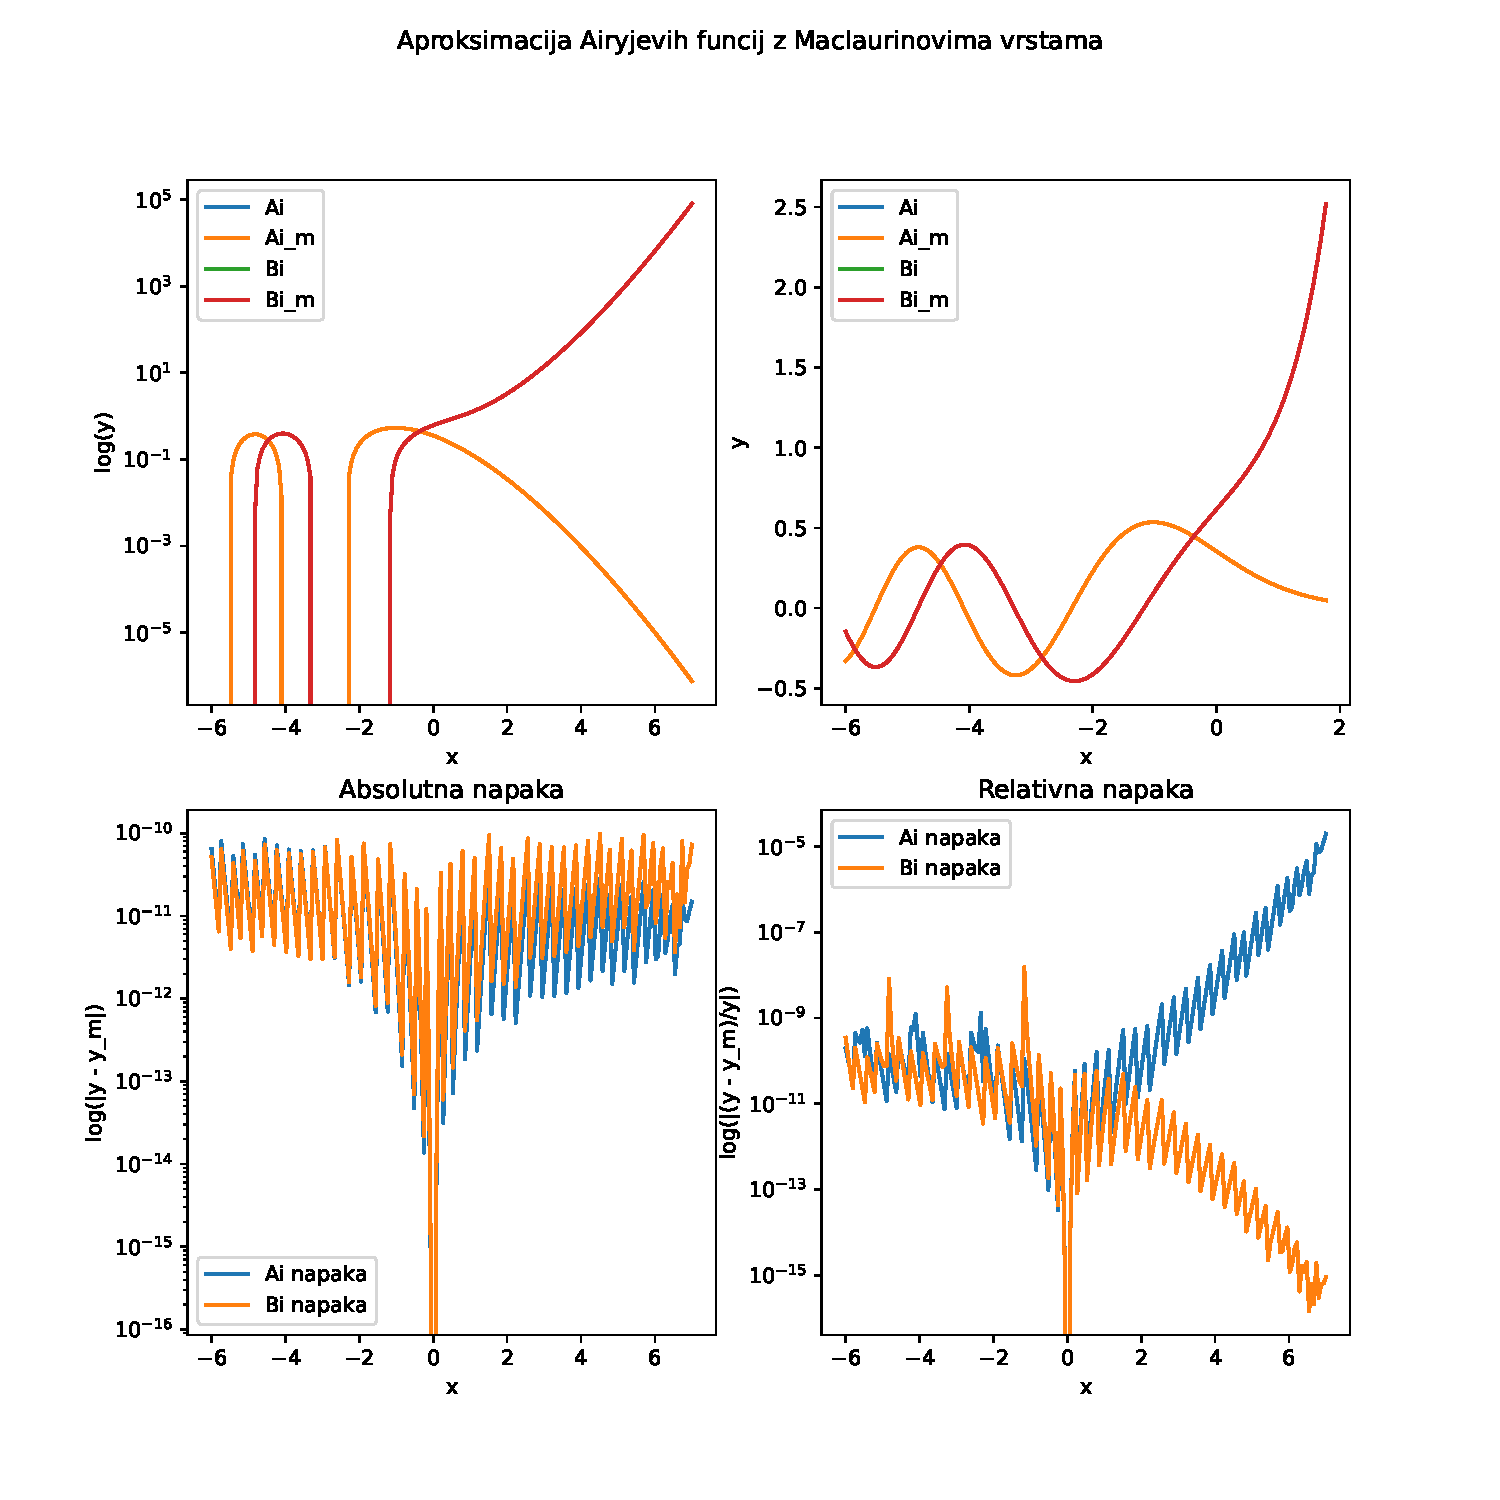
\includegraphics[width=15cm]{aprox_z_vrsto.pdf}
  \end{center}
  \vspace*{-7mm}
  \caption{Prva grafa prikazujeta realni in aproksimirani Airyjevi funkciji. Aproksimacija z Maclaurinovo vrsto je označena z \_m. Zadnja grafa prikazujeta absolutno in relativno napako aproksimacije.}
\end{figure}


\subsection{Aproksimacija Airyjevih funkcij z uporabo asimptotskih vrst}

Za velike vrednosti $|x|$ lahko Airyjevi funkciji aproksimiramo z uporabo asimptotskega razvoja navedenega v uvodu.
Aproksimacijo lahko implementiramo po definiciji, vendar s tem izgubimo nekaj natančnosti 
zaradi uporabe $\Gamma$ funkcije. Za hitrejšo in numerično bolj stabilno implementacijo
lahko uporabimo naslednjo lastnost $\Gamma$ funkcije:

\begin{equation*}
  \Gamma \left(\frac{1}{2}+n\right) = \frac{(2n)!\sqrt{\pi}}{4^n n!}
\end{equation*}

Podobno kot v prejšnjem delu lahko tu funkcije $L$, $P$ in $Q$ izrazimo rekurzivno, $L = \sum_{n=0}^{\infty} L_n , \quad L_n = l_n L_{n-1}$. Dobljene količnike ($l_n$, $p_n$ in $q_n$) lahko nato poenostavimo

\begin{align*}
  l_n &= \frac{1}{z}\left(-\frac{1}{2}+\frac{5}{72n}+\frac{n}{2}\right),\quad &L_0 &= 1 \\
  p_n &= -\frac{1}{z^2}\left(\frac{41}{72}-\frac{385}{10368n}-\frac{3n}{2}+n^2+\frac{25}{5184(2n-1)}\right),\quad &P_0 &= 1 \\
  q_n &= -\frac{1}{z^2}\left(\frac{25+288n^2(72n^2-13)}{10368n(1+2n)}\right),\quad &Q_0 &= \frac{5}{72z}
\end{align*}

S tem smo ne-elementarne funkcije pretvorili na elementarne kar izboljša časovno in numerično učinkovitost. 
Za doseganje še večje natančnosti lahko namesto 64 bitnega zapisa števil uporabimo 128 bitnega ({\sc np.float128}).

Dodatna natančnost nam omogoča doseči nekaj redov nižjo napako, predvsem pri $Bi$ za pozitivna števila. Ker funkcija tako hitro narašča števil hitro postanejo prevelika za shranjevanje. Dodatne člene v zaporedju tudi ne moremo izračunati dovolj natančno, da bi se skladali z dejansko vrednostjo. Zato absolutna napaka narašča eksponentno, čeprav bi pričakovali, da se napaka pri $x\rightarrow\infty$ bliža ničli. Relativna napaka pa hitro pade proti ničli, kar razumljivo saj so prve signifikantne števke zmeraj natančne. Funkcija $Ai$ eksponentno pada proti ničli, zato tudi napaka hitro pada.

Pri negativnih številih imamo manj težav z natančnostjo saj se tam funkcija giblje na intervalu $[-0.4, 0.4]$. Aproksimacija divergira pri izhodišču kar je skladno s teorijo.

Število členov vsote za dane rezultate je okoli 10.

\begin{figure}[hbtp]
  \begin{center}
  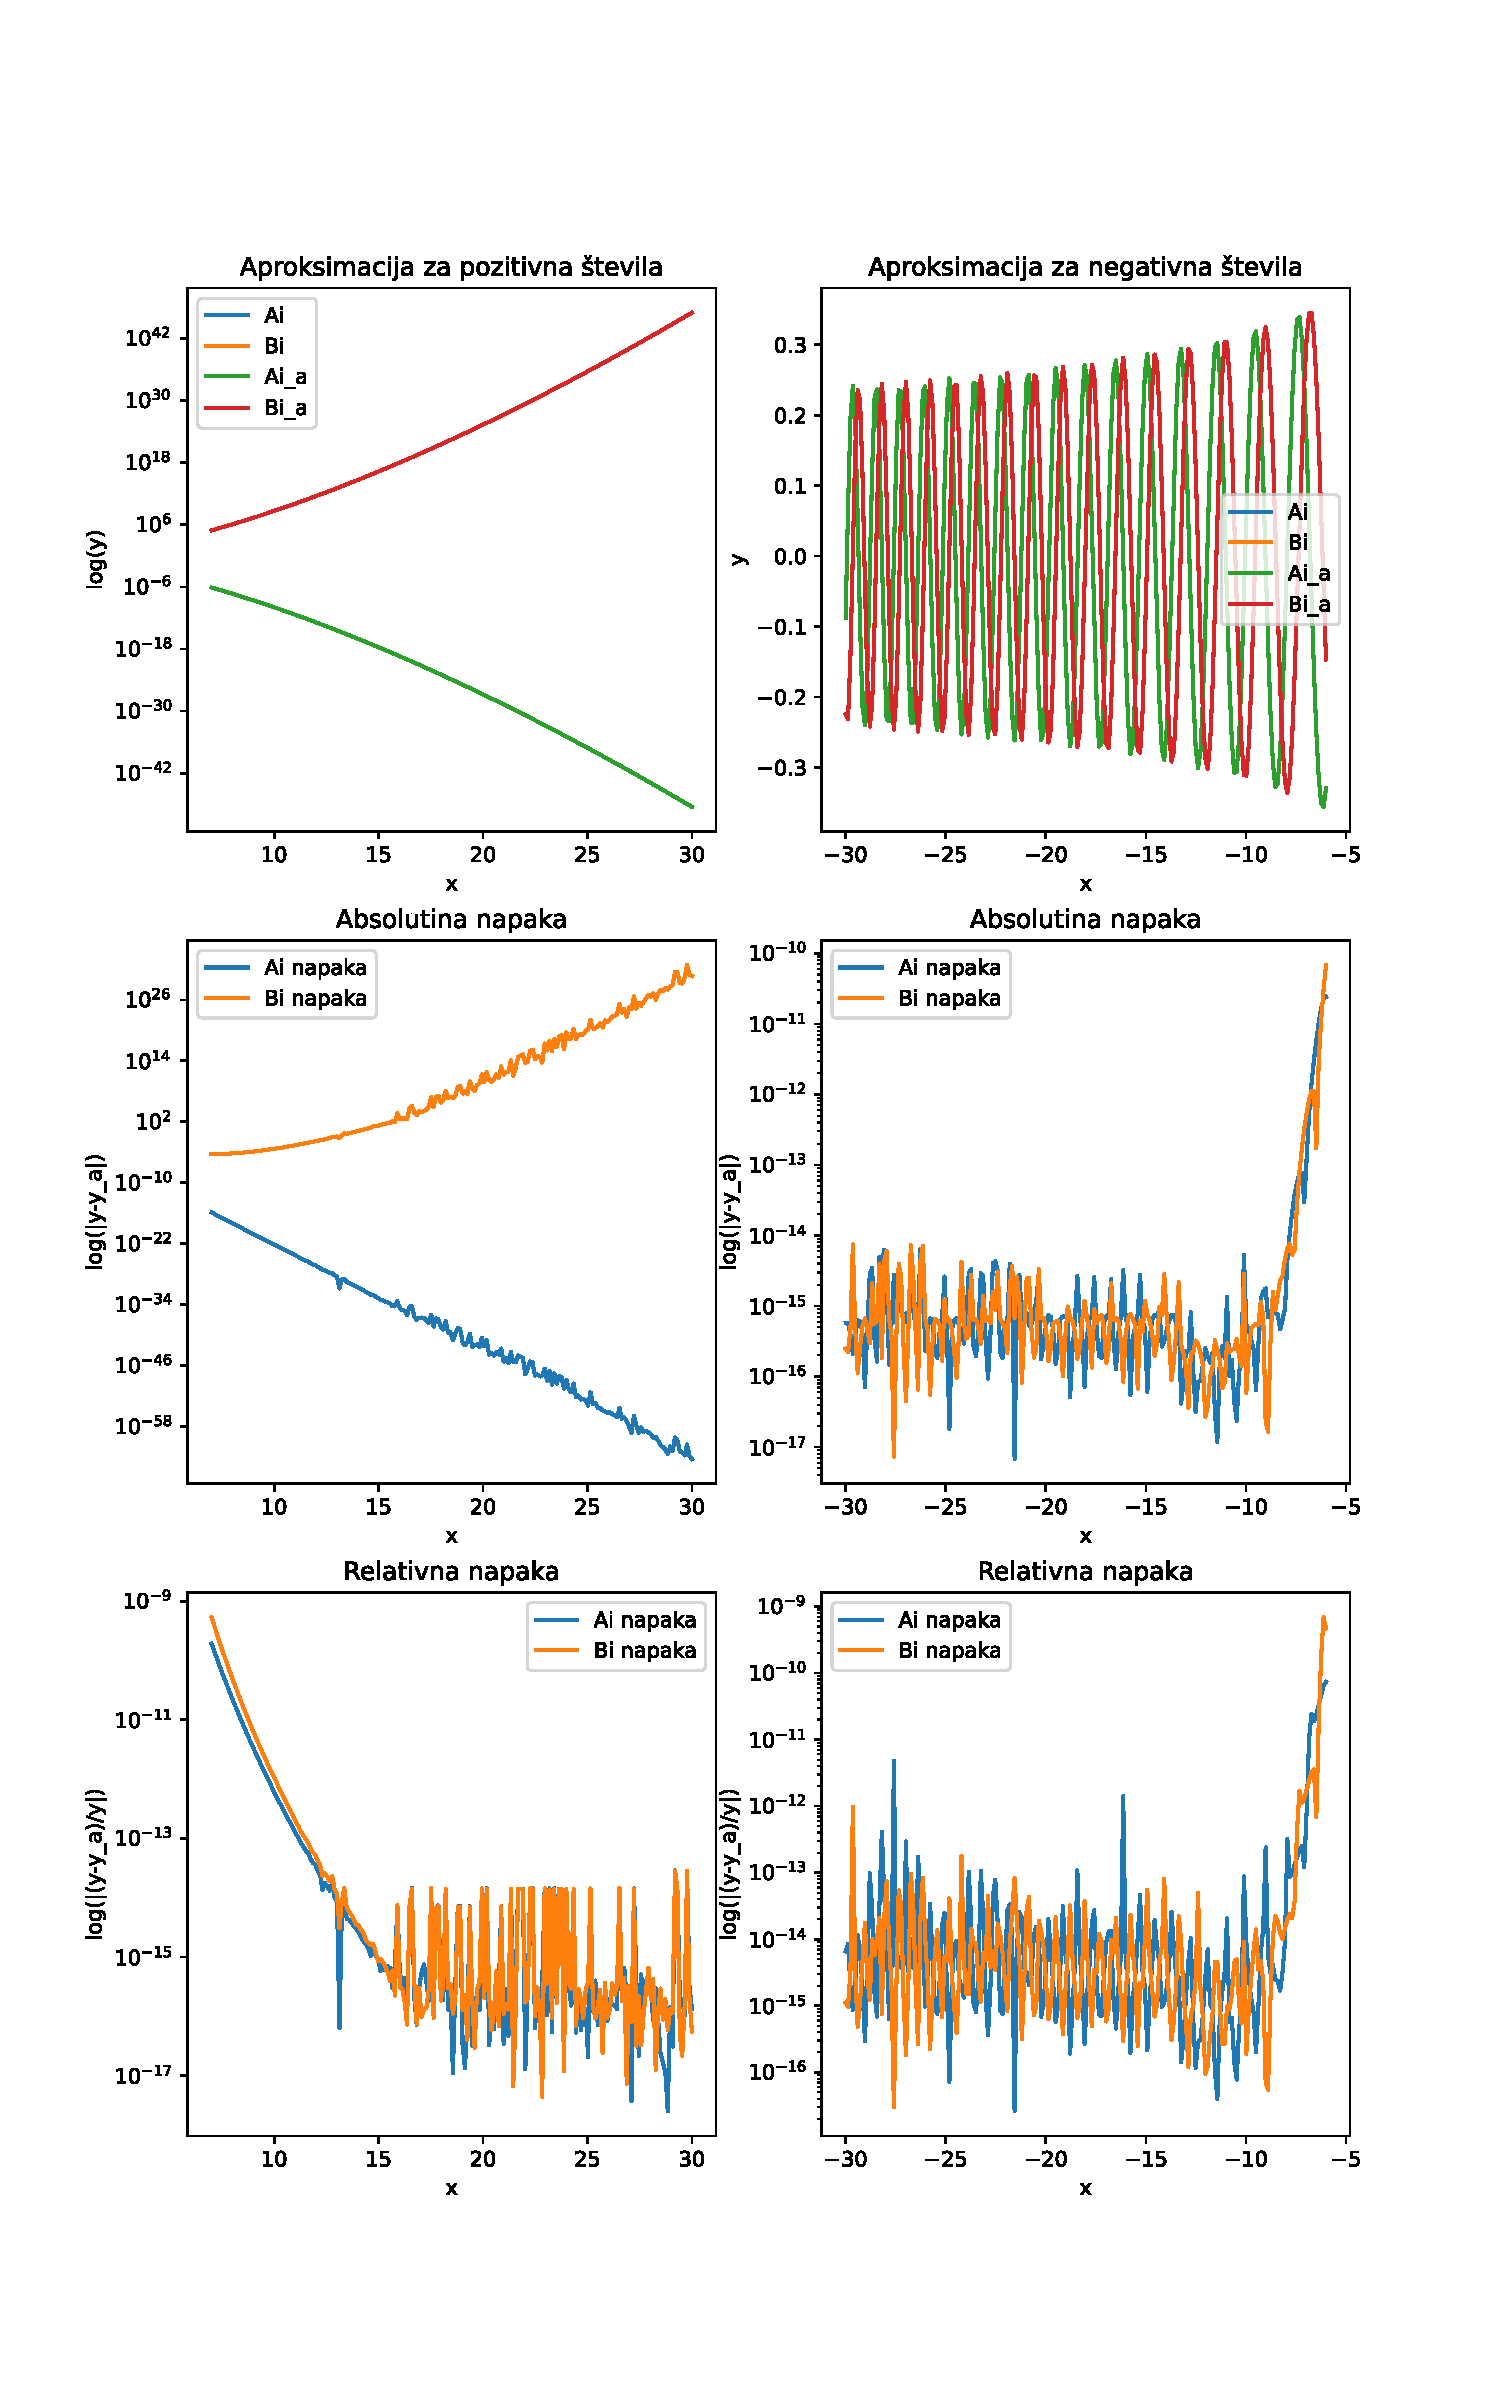
\includegraphics[width=14cm]{aprox_z_asimp_vrsto.pdf}
  \end{center}
  \vspace*{-7mm}
  \caption{Aproksimacija z asimptotskimi vrstami. Levi grafi prikazujejo aproksimacijo za pozitivna števila, desni pa za negativna.}
\end{figure}

\subsection{Zlepek približkov}

Za aproksimacijo Airyjevih funkcij na celotnem definicijskem območju moramo vse približke nekako združiti. Le-to bomo storili s primerjavo absolutnih in relativnih napak obeh približkov. Graf 3 nam podaja to primerjavo. Približek z Maclaurinovo vrsto je za $Ai$ natančen na intervalu $[-5, 4.5]$, za $Bi$ pa na $[-5, 6]$. Komplement teh intervalov aproksimiramo z asimptotskimi vrstami.

\begin{figure}[hbtp]
  \begin{center}
  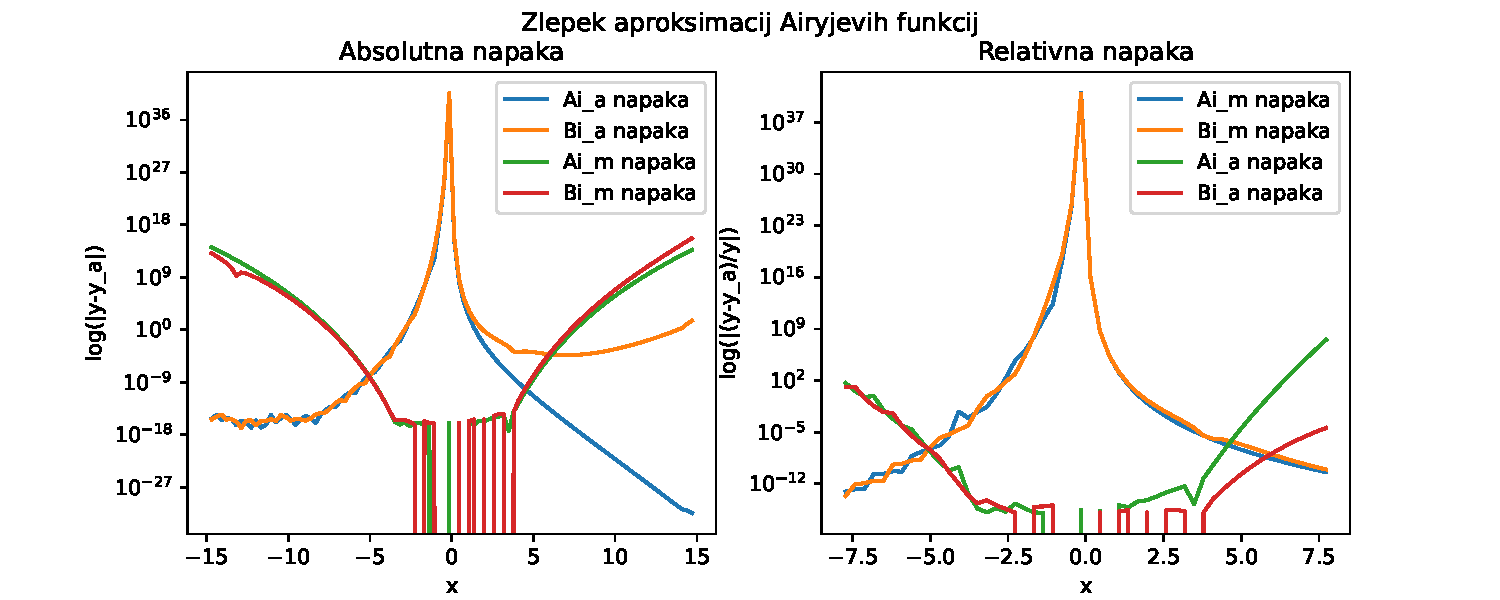
\includegraphics[width=15cm]{zlepek.pdf}
  \end{center}
  \vspace*{-7mm}
  \caption{Absolutna in relativna napaka obeh približkov na celotnem definicijskem območju.}
\end{figure}


\subsection{Ničle Airyjevih funkcij}
Poišči prvih sto ničel $\{a_s\}_{s=1}^{100}$ Airyjeve
funkcije $Ai$ in prvih sto ničel $\{b_s\}_{s=1}^{100}$
funkcije $Bi$ pri $x<0$ lahko določimo z naslednjima formulama
%
\begin{equation*}
  a_s = - f \left( \frac{3\pi(4s-1)}{8} \right), \qquad
  b_s = - f \left( \frac{3\pi(4s-3)}{8} \right), \qquad s = 1,2,\ldots \>,
\end{equation*}
%
kjer ima funkcija $f$ asimptotski razvoj
%
\begin{equation*}
  f(z) \sim z^{2/3} \left(
  1 + \frac{5}{48} \, z^{-2}
  -\frac{5}{36} \, z^{-4}
  +\frac{77125}{82944} \, z^{-6}
  -\frac{108056875}{6967296} \, z^{-8} + \ldots\right) \>.
\end{equation*}

\begin{figure}[hbtp]
  \begin{center}
  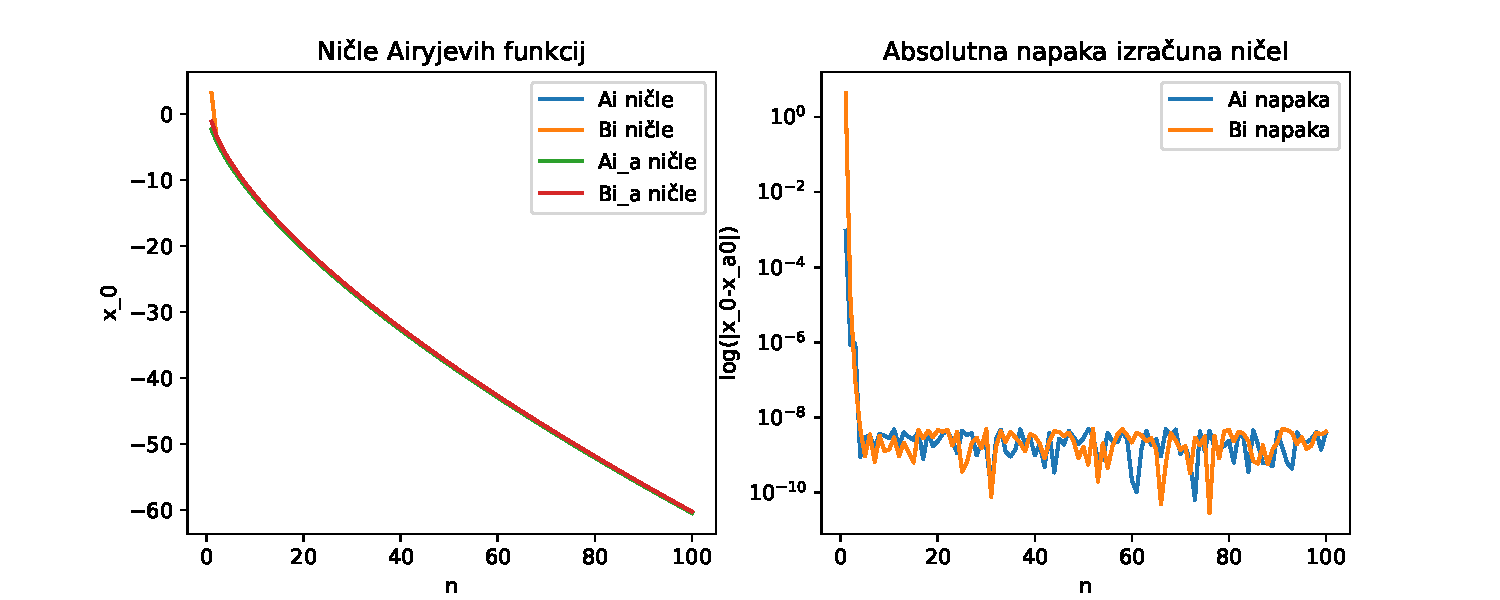
\includegraphics[width=15cm]{nicle_Airyjevih_funkcij.pdf}
  \end{center}
  \vspace*{-7mm}
  \caption{Ničle Airyjevih funkcij in absolutna napaka izračuna ničel.}
\end{figure}

Ničle lahko določimo tudi z različnimi numeričnimi metodami.
Večina teh metod potrebuje začeten približek ničle, katerega lahko dobimo z izračunom funkcije v več mestih ($N > N_{nicel}$). Približke nato uporabimo za izračun bolj natančne vrednosti ničle, kar smo v tem primeru naredili z metodo {\sc scipy.optimize.fsolve}. 
Dana metod dosega natančnost $1.49 \times 10^{-8}$, kar lahko opazimo na Grafu 4. Bolj natančno vrednost bi lahko nato dobili z bisekcijo. Odstopanje opazimo pri prvi ničli $Bi$, kjer zgornja formula da pozitivno ničlo, kar pa je napačno. Namesto zgornjih formul bi lahko zato uporabili vgrajeno funkcijo $airy$ in zgornjo numerično metodo.

\section{Zaključek}
Cilj naloge je bilo proučiti obnašanje približkov Airyjevih funkcij na celotnem definicijskem območju. 
Analiza je pokazala, da lahko z modulom {\sc numpy} dosežemo želeno natančnost, tako absolutno kot relativno napako lahko zmanjšamo na želeno toleranco. Problem nastopi pri velikih vrednostih funkcije $Bi$, ki eksponentno narašča. 
V tem primeru absolutna napaka narašča eksponentno, medtem ko se relativna manjša in hitro pade na natančnost sistema. S pametno implementacijo aproksimacijskih formul smo zmanjšali časovno zahtevnost rešitve, ker nam nato olajša iskanje ničel in poveča število členov v zaporedju. 

\end{document}

